

\title{Predefined Styles}
\author{Lorenzo Pichetti}
\date{2021}

\documentclass{article}
\usepackage{float}
    
% ========== Tikz setting ==========
%\usepackage[svgnames]{xcolor}
\usepackage{tikz}
\usetikzlibrary{decorations.markings}
\usetikzlibrary{shapes.geometric}
\pagestyle{empty}

\pgfdeclarelayer{edgelayer}
\pgfdeclarelayer{nodelayer}
\pgfsetlayers{edgelayer,nodelayer,main}

\tikzstyle{none}=[inner sep=0pt]

\tikzstyle{red}=[circle,fill=red,draw=black,line width=0.8 pt]
\tikzstyle{green}=[circle,fill=lime,draw=black,line width=0.8 pt]
\tikzstyle{yellow}=[circle,fill=yellow,draw=black,line width=0.8 pt]
\tikzstyle{black}=[circle,fill=black,draw=black]
\tikzstyle{white}=[circle,fill=white,draw=black]
\tikzstyle{little}=[circle,fill=gray,draw=gray,scale=0.5 pt]

\tikzstyle{simple}=[-,draw=white,line width=3.000]
\tikzstyle{arrow}=[->,draw=darkgray,line width=2.000]
\tikzstyle{tick}=[-,draw=black,postaction={decorate},decoration={markings,mark=at position .5 with {\draw (0,-0.1) -- (0,0.1);}},line width=2.000]
\tikzstyle{redstyle}=[-,draw=red,line width=3.000]
\tikzstyle{bluestyle}=[-,draw=blue,line width=3.000]
\tikzstyle{greenstyle}=[-,draw=lime,line width=3.000]
\tikzstyle{flow}=[->,draw=green,line width=2.000]
\tikzstyle{redarrow}=[-latex,draw=red,line width=3.000]
\tikzstyle{greenarrow}=[-latex,draw=green,line width=3.000]
\tikzstyle{bluearrow}=[-latex,draw=blue,line width=3.000]
\tikzstyle{axe}=[->,draw=black,line width=2.000]
\tikzstyle{thiny}=[-,draw=lightgray,line width=1.000]

\usepackage{tikzscale}


\begin{document}

\maketitle
    
\section{Predefined styles}
In this file we show all the predefined styles for nodes and edges. Other styles can be defined by adding its definition inside the function \textit{print\_preambles} into \textit{LatexGraph.py}.
    
	\subsection{Nodes styles}
	
	\begin{figure}[H]
		\begin{center}
			\resizebox{0.95\textwidth}{!}{
				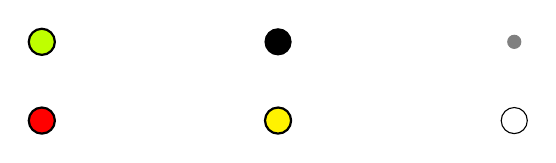
\begin{tikzpicture}
					\begin{pgfonlayer}{nodelayer}
						\node [style=red] (0) at (0.000,0.000) {};
						\node [style=green] (1) at (0.000,1.000) {};
						\node [style=yellow] (3) at (3.000,0.000) {};
						\node [style=black] (4) at (3.000,1.000) {};
						\node [style=white] (6) at (6.000,0.000) {};
						\node [style=little] (7) at (6.000,1.000) {};
					\end{pgfonlayer}
					\begin{pgfonlayer}{edgelayer}
					\end{pgfonlayer}
				\end{tikzpicture}
			}
		\end{center}
		\caption{These are all the predefined node styles; in the first line, from left to right we have \textit{'green'}, \textit{'black'}, and \textit{'little'}, on the second line \textit{'red'}, \textit{'yellow'}, and \textit{'white'}.}
		\label{fig:lat1a}
	\end{figure}
	
	\subsection{Edges styles}
	
	\begin{figure}[H]
		\begin{center}
			\resizebox{0.95\textwidth}{!}{
				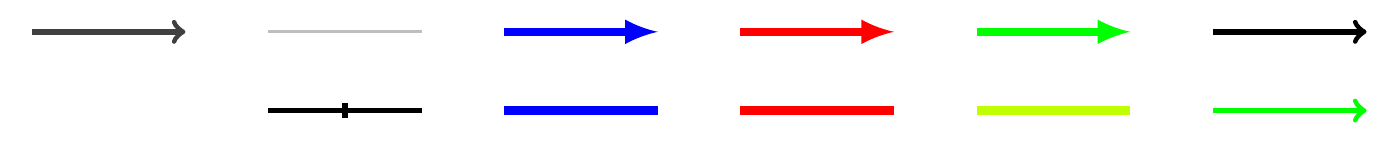
\begin{tikzpicture}
					\begin{pgfonlayer}{nodelayer}
						\node [style=none] (simple) at (0.000,0.000) {};
						\node [style=none] (simple0) at (2.000,0.000) {};
						\node [style=none] (arrow) at (0.000,1.000) {};
						\node [style=none] (arrow0) at (2.000,1.000) {};
						\node [style=none] (tick) at (3.000,0.000) {};
						\node [style=none] (tick0) at (5.000,0.000) {};
						\node [style=none] (thiny) at (3.000,1.000) {};
						\node [style=none] (thiny0) at (5.000,1.000) {};
						\node [style=none] (bluestyle) at (6.000,0.000) {};
						\node [style=none] (bluestyle0) at (8.000,0.000) {};
						\node [style=none] (bluearrow) at (6.000,1.000) {};
						\node [style=none] (bluearrow0) at (8.000,1.000) {};
						\node [style=none] (redstyle) at (9.000,0.000) {};
						\node [style=none] (redstyle0) at (11.000,0.000) {};
						\node [style=none] (redarrow) at (9.000,1.000) {};
						\node [style=none] (redarrow0) at (11.000,1.000) {};
						\node [style=none] (greenstyle) at (12.000,0.000) {};
						\node [style=none] (greenstyle0) at (14.000,0.000) {};
						\node [style=none] (greenarrow) at (12.000,1.000) {};
						\node [style=none] (greenarrow0) at (14.000,1.000) {};
						\node [style=none] (flow) at (15.000,0.000) {};
						\node [style=none] (flow0) at (17.000,0.000) {};
						\node [style=none] (axe) at (15.000,1.000) {};
						\node [style=none] (axe0) at (17.000,1.000) {};
					\end{pgfonlayer}
					\begin{pgfonlayer}{edgelayer}
						\draw [style=simple] (simple) to (simple0);
						\draw [style=arrow] (arrow) to (arrow0);
						\draw [style=tick] (tick) to (tick0);
						\draw [style=thiny] (thiny) to (thiny0);
						\draw [style=bluestyle] (bluestyle) to (bluestyle0);
						\draw [style=bluearrow] (bluearrow) to (bluearrow0);
						\draw [style=redstyle] (redstyle) to (redstyle0);
						\draw [style=redarrow] (redarrow) to (redarrow0);
						\draw [style=greenstyle] (greenstyle) to (greenstyle0);
						\draw [style=greenarrow] (greenarrow) to (greenarrow0);
						\draw [style=flow] (flow) to (flow0);
						\draw [style=axe] (axe) to (axe0);
					\end{pgfonlayer}
				\end{tikzpicture}
			}
		\end{center}
		\caption{These are all the predefined edges styles; from left to right in the first line we have \textit{'arrow'}, \textit{'thiny'}, \textit{'bluearrow'}, \textit{'redarrow'}, \textit{'greenarrow'}, and \textit{'axse'}, and in the second line \textit{'simple'}, \textit{'tick'}, \textit{'bluestyle'}, \textit{'redstyle'}, \textit{'greenstyle'}, and \textit{'flow'}.}
		\label{fig:lat1a}
	\end{figure}
	
\end{document}
